\documentclass{article}
\usepackage[dvipsnames]{xcolor}
\usepackage[utf8]{inputenc}
\usepackage{url}
\usepackage{amsmath}
\usepackage{amssymb}
\usepackage{graphicx}
\usepackage{tikz}
\usepackage{subfig}
\usetikzlibrary{positioning}
\usepackage{caption}
\usepackage{hyperref}
\usepackage{xcolor}
\hypersetup{
    colorlinks=true,
    linkcolor=blue,
    filecolor=magenta,      
    urlcolor=blue,
    pdftitle={Git tips},
}

\title{Some (hopefully) helpful tips for using git}
\author{\href{https://www.linkedin.com/in/mkrajewski14/}{Mateusz Krajewski}}

\begin{document}

\maketitle
\tableofcontents
\newpage

\section{Introduction} 
It is of paramount importance that we use git in an organised and consistent manner. It will reduce confusion and make it easier to mitigate the consequences of our mistakes. And there will be plenty, inevitably. The following is my attempt to standardise our git workflow. Feel free to share this document and adjust it to Your needs -- just remember to keep my name in. \hyperref[sec:contributing]{Contributions} will be appreciated.

In order to make the branch history as clean as possible, we have decided to create seven separate branches - one for every team member. Every developer is going to work on their issues on the branch assigned to them - and merge it with main when necessary.

I am going to present a couple of common scenarios that can arise when working with git. I tried to make it as relatable to the current project as possible. For that reason, all the examples below are based solely in Eclipse IDE. I may include some command-line examples later on.

\section{The development process}

The following is the general overview of our development process. You should try to adhere to it as much as possible. To explore the steps in more details, refer to the later parts of this document.

\begin{enumerate}
	\item Start working on the issue on Your own branch.
	\item Remember to commit and push regularly, so that other team members can review Your changes.
	\item Your work is only done when Your code reviewer says so.
	\item In order to merge, first make sure that Your local main branch is up-to-date with the remote one. \hyperref[sec:switching]{Switch} to main and \hyperref[sec:pulling]{pull} from the remote.
	\item Then, \hyperref[sec:merging]{merge} Your branch into main. Solve any \hyperref[sec:conflicts]{conflicts} that may arise.
	\item Close the issue in the issue tracker.
\end{enumerate}

\section{Miscellany}

\subsection{Git staging}
\label{sec:git_staging}

There are two helpful views that You can enable in order to better understand what's going on. One of them is \textit{Git staging}. You'll find it in: \newline

$\mathtt{Window\rightarrow Show\ view \rightarrow Other \rightarrow Git \rightarrow Git\ Staging}$.\newline

It's an easy tool for reviewing the changes You have made, and ultimately committing them.

\subsection{History}
\label{sec:git_history}

You can find \textit{History} view under: \newline

$\mathtt{Window \rightarrow Show\ view \rightarrow Other \rightarrow Team \rightarrow History}$.\newline

It shows the history of changes made to the chosen resource in the \textit{Package Explorer}. Besides, it makes it extremely simple to see the state of current branches, both local and remote.

\subsection{Current branch}

The branch You're currently in is displayed right next to the project name in \textit{Package Explorer} (Figure  \ref{fig:branch_name}). You almost certainly know this. But if I want to make this document as comprehensive as possible, it needs to be here.

\begin{figure}[h]
    \centering
    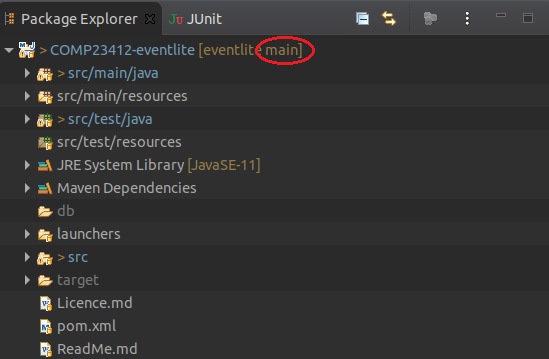
\includegraphics[scale=0.6]{branch_name.png}
    \caption{The location of the current branch name.}
    \label{fig:branch_name}
\end{figure}

\subsection{Pulling}
\label{sec:pulling}

In order to synchronise Your local branch with any changes made to its remote counterpart, right-click the project name and select:\newline

$\mathtt{Team \rightarrow Pull}$. \newline

Most likely, You will have to choose between two identical \textit{Pull} options. The only difference is that the second one goes into the process in more detail. Ultimately, though, it doesn't really matter which one You'll pick.

\section{Moving between branches}
\label{sec:switching}

This is probably basic knowledge as well. In Eclipse, You can switch between branches/commits by right-clicking the project name in the \textit{Package Explorer} and choosing:\newline

$\mathtt{Team \rightarrow Switch\ to}$.\newline

With the help of this tool, it is possible to:

\begin{itemize}
    \item Create a new local branch;
    \item Create a local copy of a remote branch;
    \item Switch between local branches;
    \item Switch between commits.
\end{itemize}

\textbf{NOTE: } Before You do any of that, make sure to look into \hyperref[sec:git_staging]{Git staging} and commit any changes You have made so far. Otherwise, git may behave unpredictably and You will spend the next two hours trying to figure out what to do (it certainly never happened to me, duh). 

\section{Updating the feature branch}

Suppose You started working on Your branch and already made some commits. In the meantime, however, one of Your teammates merged their work into main and now Your branch is outdated. In such a case, the commit graph may look (roughly) like in Figure \ref{fig:before_update}. You may want to update Your branch and keep working on it, without having to merge into main (not yet, at least). In order to do that, You can do the opposite - merge main into Your branch. This operation would result in creating a new merge commit, just like in Figure \ref{fig:after_update}.\newline

\begin{minipage}[b]{0.45\textwidth}
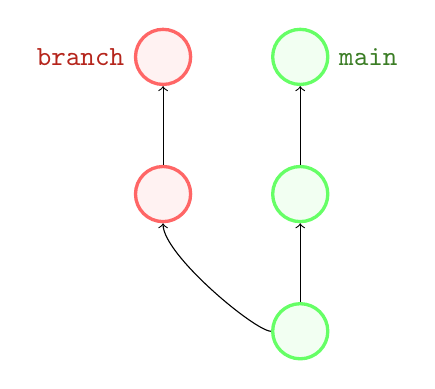
\begin{tikzpicture}[
    mainnode/.style={circle, draw=green!60, fill=green!5, very thick, minimum size=7mm},
    branchnode/.style={circle, draw=red!60, fill=red!5, very thick, minimum size=7mm}
]
\node[mainnode](main){};
\node[mainnode](main2)[above=of main]{};
\node[mainnode](main3)[above=of main2, label=right:\textcolor{OliveGreen}{$\mathtt{main}$}]{};
\node[branchnode](branch)[left=of main2]{};
\node[branchnode](branch2)[above=of branch, label=left:\textcolor{BrickRed}{$\mathtt{branch}$}]{};
\draw[->] (main.north) -- (main2.south);
\draw[->] (main2.north) -- (main3.south);
\draw[->] (main.west) .. controls +(left:2mm) and +(down:4mm) .. (branch.south);
\draw[->] (branch.north) -- (branch2.south);
\end{tikzpicture}
\captionof{figure}{Before updating.}
\label{fig:before_update}
\end{minipage}
\hspace{0.1\textwidth}
\begin{minipage}[b]{0.45\textwidth}
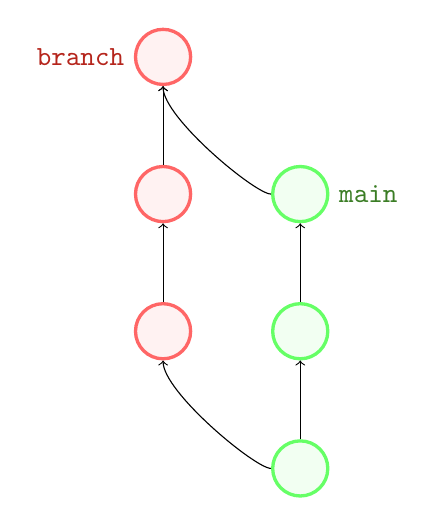
\begin{tikzpicture}[
    mainnode/.style={circle, draw=green!60, fill=green!5, very thick, minimum size=7mm},
    branchnode/.style={circle, draw=red!60, fill=red!5, very thick, minimum size=7mm}
]
\node[mainnode](main){};
\node[mainnode](main2)[above=of main]{};
\node[mainnode](main3)[above=of main2, label=right:\textcolor{OliveGreen}{$\mathtt{main}$}]{};
\node[branchnode](branch)[left=of main2]{};
\node[branchnode](branch2)[above=of branch]{};
\node[branchnode](branch3)[above=of branch2, label=left:\textcolor{BrickRed}{$\mathtt{branch}$}]{};
\draw[->] (main.north) -- (main2.south);
\draw[->] (main2.north) -- (main3.south);
\draw[->] (main.west) .. controls +(left:2mm) and +(down:4mm) .. (branch.south);
\draw[->] (branch.north) -- (branch2.south);
\draw[->] (branch2.north) -- (branch3.south);
\draw[->] (main3.west) .. controls +(left:2mm) and +(down:4mm) .. (branch3.south);
\end{tikzpicture}
\captionof{figure}{After updating.}
\label{fig:after_update}
\end{minipage}

\paragraph{}
Now, how to do that? The process itself is quite simple. First, make sure that the main branch is synchronised with the remote (\hyperref[sec:switching]{switch} to main and \hyperref[sec:pulling]{pull}). Then, \hyperref[sec:switching]{switch} to the feature branch. Right-click the project name and choose the following:\newline

$\mathtt{Team\rightarrow Merge}.$\newline

After that, select the local main branch. Solve any \hyperref[sec:conflicts]{conflicts} that may arise. Move on.

\section{Merging with main}
\label{sec:merging}
Merging is really quite simple. Before You do that, however, make sure that Your main branch is up-to-date with the remote one (\hyperref[sec:switching]{switch} to main and \hyperref[sec:pulling]{pull} the remote). After that, right-click the project name and choose:\newline

$\mathtt{Team\rightarrow Merge}$.\newline

Then, select the branch You want to merge into main. No need to meddle with the additional options. Now, if we imagine a commit graph like that in Figure \ref{fig:before_update}, its structure after the merge would be similar to that in Figure \ref{fig:after_merge}. Note how git creates an additional merge commit, which incorporates the changes made both in the main branch and in the feature branch. Any further changes made to the feature branch will result in the graph evolving like in Figure \ref{fig:after_changes}.

If You encounter conflicts, refer to section \ref{sec:conflicts}.\newline

\begin{minipage}[b]{0.45\textwidth}
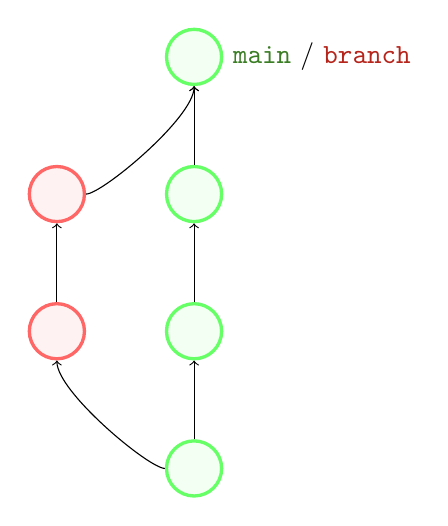
\begin{tikzpicture}[
    mainnode/.style={circle, draw=green!60, fill=green!5, very thick, minimum size=7mm},
    branchnode/.style={circle, draw=red!60, fill=red!5, very thick, minimum size=7mm}
]
\node[mainnode](main){};
\node[mainnode](main2)[above=of main]{};
\node[mainnode](main3)[above=of main2]{};
\node[mainnode](main4)[above=of main3, label=right:\textcolor{OliveGreen}{$\mathtt{main}$} / \textcolor{BrickRed}{$\mathtt{branch}$}]{};
\node[branchnode](branch)[left=of main2]{};
\node[branchnode](branch2)[above=of branch]{};
\draw[->] (main.north) -- (main2.south);
\draw[->] (main2.north) -- (main3.south);
\draw[->] (main3.north) -- (main4.south);
\draw[->] (main.west) .. controls +(left:2mm) and +(down:4mm) .. (branch.south);
\draw[->] (branch.north) -- (branch2.south);
\draw[->] (branch2.east) .. controls +(right:2mm) and +(down:4mm) .. (main4.south);
\end{tikzpicture}
\captionof{figure}{After merge.}
\label{fig:after_merge}
\end{minipage}
\hspace{0.1\textwidth}
\begin{minipage}[b]{0.45\textwidth}
\begin{tikzpicture}[
    mainnode/.style={circle, draw=green!60, fill=green!5, very thick, minimum size=7mm},
    branchnode/.style={circle, draw=red!60, fill=red!5, very thick, minimum size=7mm}
]
\node[mainnode](main){};
\node[mainnode](main2)[above=of main]{};
\node[mainnode](main3)[above=of main2]{};
\node[mainnode](main4)[above=of main3, label=right:\textcolor{OliveGreen}{$\mathtt{main}$}]{};
\node[branchnode](branch)[left=of main2]{};
\node[branchnode](branch2)[above=of branch]{};
\node[branchnode](branch3)[above=of branch3, label=left:\textcolor{BrickRed}{$\mathtt{branch}$}]{};
\draw[->] (main.north) -- (main2.south);
\draw[->] (main2.north) -- (main3.south);
\draw[->] (main3.north) -- (main4.south);
\draw[->] (main.west) .. controls +(left:2mm) and +(down:4mm) .. (branch.south);
\draw[->] (branch.north) -- (branch2.south);
\draw[->] (branch2.east) .. controls +(right:2mm) and +(down:4mm) .. (main4.south);
\draw[->] (main4.west) .. controls +(left:2mm) and +(down:4mm) .. (branch3.south);
\end{tikzpicture}
\captionof{figure}{After further changes.}
\label{fig:after_changes}
\end{minipage}

\section{Solving conflicts}
\label{sec:conflicts}

Merge conflicts are inevitable. No matter what You're trying to achieve by merging, they will often be there. And they will need to be solved. A conflict is signified by a window similar to that in figure \ref{fig:conflict_message}.

\begin{figure}[h]
	\centering
	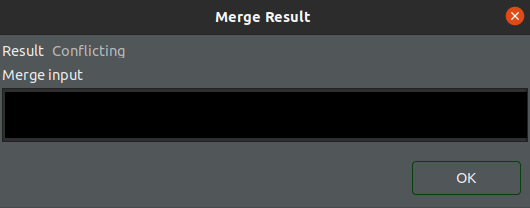
\includegraphics[scale=0.6]{conflict_message.png}
	\caption{A conflict message.}
	\label{fig:conflict_message}
\end{figure}

The \textit{Unstaged changes} section in \hyperref[sec:git_staging]{Git Staging} lists all files where conflicts were detected (Figure \ref{fig:staging_conflicts}). Successfully merged files are in the \textit{Staged changes} section. Now, every conflict can be solved in two ways - either manually or by using a \textit{Merge Tool}.

\begin{figure}[h]
	\centering
	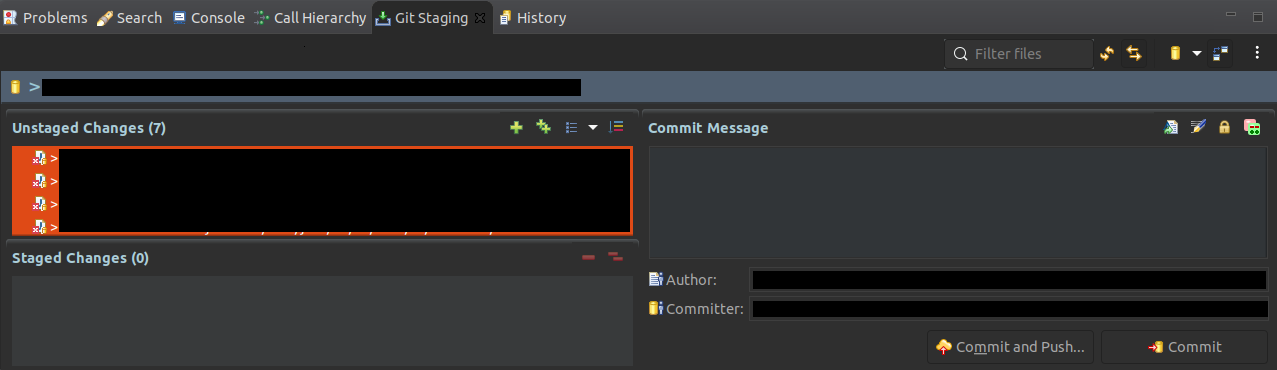
\includegraphics[scale=0.27]{staging_conflicts.png}
	\caption{\hyperref[sec:git_staging]{Git Staging} view during a merge conflict.}
	\label{fig:staging_conflicts}
\end{figure}

\subsection{Manually}
Following the hints from \hyperref[sec:git_staging]{Git Staging}, find and open the respective files in the \textit{Package Explorer}. Every conflict would be of the form:
\begin{verbatim}
<<<<<<< HEAD
what you see in the branch You're merging into
=======
what you see in Your branch
>>>>>>>
\end{verbatim}
Modify this part in the way You deem appropriate (remember to remove the redundant symbols), and then \textbf{immediately} save and stage the changes. Move on to the next file.

\subsection{With a \textit{Merge Tool}}
The \textit{Merge Tool} can be opened either by selecting the conflicting files in \hyperref[sec:git_staging]{Git Staging} or right-clicking the project name in the \textit{Package Explorer} and choosing:\newline

$\mathtt{Team \rightarrow Merge\ Tool}$.\newline

There are two main sections in the \textit{Merge Tool}. The left one shows what the files look like in the branch You're merging into. This is where You apply Your changes. The right one shows what the files look like in Your branch. You can't change anything here.	

The \textit{Merge Tool} highlights all differences between the two files. Use it to Your advantage:
\begin{itemize}
	\item \textbf{\textcolor{blue}{Blue}} - the change exists in Your branch, doesn't exist in the branch You're merging into;
	\item \textbf{\textcolor{green}{Green}} - the change doesn't exist in Your branch, exists in the branch You're merging into;
	\item \textbf{\textcolor{red}{Red}} - both Your branch and the branch You're merging into have applied different changes to the same segment, and they can't be combined together;
	\item \textbf{\textcolor{darkgray}{Grey}} - both Your branch and the branch You're merging into have applied different changes to the same segment, but they can be combined together. 
\end{itemize}

Every time You finish applying changes to the given file, \textbf{immediately} save and stage them. Once You're done, commit the changes. The merge commit message will be generated automatically.

\section{Git commit messages}
\label{sec:commit_messages}
I know it's hard, but it is very important to make commit messages as consistent as possible. Try to follow these few simple guidelines: 
\begin{itemize}
    \item Start the message with the imperative form of the verb i.e. \textit{add, fix, delete};
    \item Begin with a capital letter; 
    \item Keep it short;
    \item Provide the concise outline of what You did;
    \item Don't end the message with a period. 
\end{itemize}

\section{Contributing}
\label{sec:contributing}
If You want to contribute, check out the \href{https://github.com/marzipan14/git_tips}{GitHub repository}.

\section{Acknowledgements}
I would like to thank \href{https://www.linkedin.com/in/zoya-anwar/}{Zoya Anwar} for her invaluable feedback.

\end{document}
